\documentclass[a4paper,12pt]{article}
\usepackage[utf8]{inputenc}
\usepackage[T1]{fontenc}
\usepackage{graphicx}
\usepackage{grffile}
\usepackage{longtable}
\usepackage{wrapfig}
\usepackage{rotating}
\usepackage[normalem]{ulem}
\usepackage{amsmath}
\usepackage{textcomp}
\usepackage{amssymb}
\usepackage[hmargin=1.42in,vmargin=1in]{geometry}
\usepackage{fontspec}
\defaultfontfeatures{Ligatures=Discretionary,Numbers=OldStyle}
\setmainfont{Palatino Linotype}
\usepackage[math-style=TeX]{unicode-math}
\setmathfont{TeX Gyre Pagella Math}
\usepackage{microtype}
\usepackage{caption}
\usepackage{hyperref}
\author{Paul R. Halmos}
\date{January 14, 1994}
\title{What is Teaching?\footnote{Talk presented at the annual meeting of The Mathematical Association of America, Cincinnati,
Ohio, 14 January 1994.}}
\hypersetup{
 pdfauthor={Paul R. Halmos},
 pdftitle={What is Teaching?},
 pdflang={English}}

\begin{document}
\maketitle

Do you remember the first time you ever taught?  The first day I taught
was September 18, 1935—which was slightly over 58 years ago, or, if you
want to be very precise, exactly 21,303 days ago today.  Does that, I
wonder, make me the person with the longest teaching experience in this
room?  Being aware of the length of my servitude, the authorities in
charge of our meeting today deduced that I know, or, in any event, I
ought to know what teaching is, and they instructed me to tell you.

The course I taught in 1935 was called freshman algebra; its purpose
was to reveal the secrets of quadratic equations (for which there was
a formula) and parentheses (which were abominable entities and had to
be eliminated at the drop of a hat).  The course met at 8:00 in the
morning, five days a week—yes, five days, Monday through Friday,
inclusive; my pay was \$45.00 a month.  Incidentally, I was living at
the time in an old-fashioned, comfortable, large, 5-room apartment,
within five minutes walk of the campus; the rent was \$45.00 a month.

I had no fear of teaching.  Stage fright, yes; fear, no.  Stage fright,
in the sense of being keyed up and slightly nervous is something that
has always been with me six minutes for each new class: five minutes
before it first meets and one minute after it starts.  The same is true
of colloquium talks and all other kinds of public appearances.

Even though there was still a lot I had to learn about teaching, I
thought I could cope with it.  I have always been surprised by beginners
who say they don’t know how to teach yet.  Haven’t they already spent
almost twenty years under the influence of teachers, and haven’t they
noticed that some techniques seem to work well and others are just
annoying, and haven’t they ever muttered to themselves “I could explain
that a lot better”?  I had had some bad teachers along with the good
ones, and I thought I knew what not to do—I marched to my first class
confidently with my head held high and with the stage fright barely
noticeable under my eagerness to get on with it.

The ages of my students were around 17 and 18; I was a wise old
graduate student aged 19.  They believed what I told them.  Some of
them were good and some of them were hopeless.  The only one whose
name I’ll never forget (it was not Drossin, but let’s call him that)
was one of the hopeless ones.  Attendance spotty, homework missing or
weak, midterm exams around D minus, the final exam might have helped
him pass the course, but I didn’t have much faith and neither did he.
The Saturday evening before the final a small party at my house was
interrupted by the doorbell—it was Drossin.  Could he speak to me a
minute, privately?  Somewhat suprised, I took him to an unused room,
and asked him what’s up.  I was a graduate student, wasn’t I?  And
perhaps I wasn’t too well off, was I?  And this course was important
for him, so he’d appreciate it if I would help him pass it, and he’d
make it worth my while—he’d give me five dollars.  Half a week’s rent,
a week’s food!  I was too surprised to be angry, but I told him to go
away.  I returned to the party and told my friends that I had just
learned how much I was worth.  Next Monday, Drossin’s paper was the
first I graded.  He flunked, with no margin for error.

\begin{figure}[htbp]
\centering
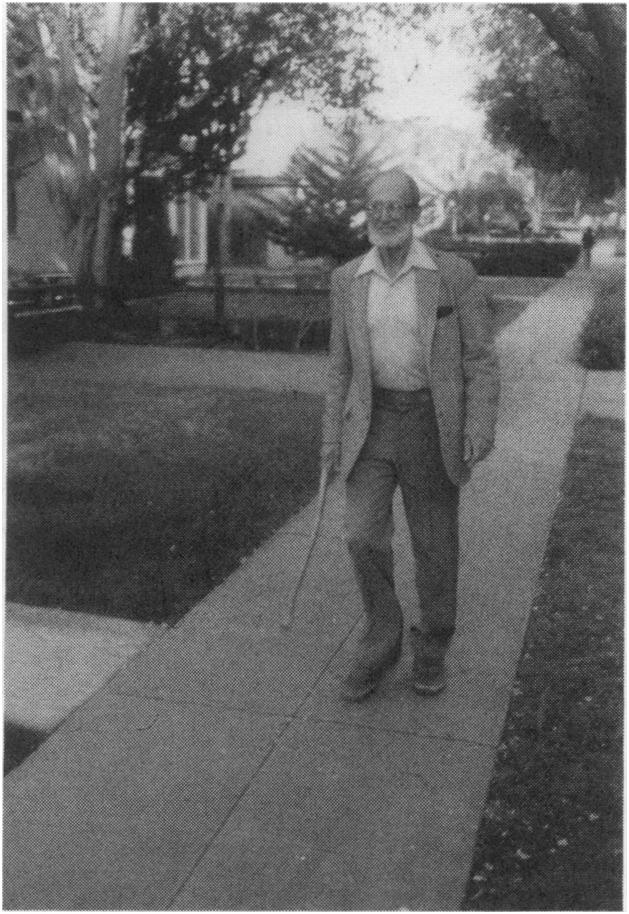
\includegraphics[width=.54\linewidth]{Halmos-Walking.png}
\caption*{\label{fig:halmos-walking}Paul Halmos engaged in one of his favorite activities.}
\end{figure}

Well, what about telling you what teaching is?  The more I tried to
think what to say, the more I was being led to the conclusion that
nobody cain’t never teach nobody nuttin’ nohow.  I don’t really mean
that, but I mean it a lot more than its opposite, and I thought I’d
get your attention more quickly by making a crisp statement.  I’ll
spend some of the rest of my time telling you which part of that
provocative crispness I really mean.

There are three types of knowledge that we commonly speak of as subjects
for teaching or learning; they can be most effectively identified as what,
how, and why.

To be educated means to remember something, to be able to use it, and to
understand it.  Frequently these three kinds of education are thought of as
belonging to altogether different kinds of human activity, but ideally they
are all present every time.  Our memory knows that Napoleon was defeated at
Waterloo, our muscles know that certain stretchings and bendings will cause
our feet to alternate suitably so as to take us from the office to lunch,
and our mind knows why three times five is the same as five times three.

Many students confuse education with memorization.  They tend to think
that if we know the boiling point of beer, the gestation period of
elephants, the conjugation of French irregular verbs, and the population
of Burma, together with many other such goodies about the moon, whales,
protons, synapses, schizophrenia, and interest rates, then we are
educated.  A walking encyclopedia is, however, rarely an educated person.
To a historian, history is not just a collection of facts but an organized
understanding of how we got to be what we are; Waterloo is not just a
fact, but, possibly, a tool to be used to avoid catastrophes in the
future.  To a chemist, chemistry is not just purple liquids in test tubes,
but a scheme for prediction and a way of understanding the world—and the
same sort of thing is true of the physicist, the astronomer, the
psychologist, and the economist.

Sometimes education is oriented toward application, only application, and
the result is just as wide of the mark.  A linguist is not one who can
speak strange languages, certainly not only that, and a cellist is not one
who knows where to put the fingers of his left hand and at what angle to
pull his right elbow back.  Etymology and syntax for the one, and
musicology and musicianship for the other play the role of the vitally
necessary components of remembering and understanding.

The third sin, that of identifying education with ratiocination is
rarer, but not unknown: the philosophers who, allegedly, don’t want to
be burdened with or confused by mere facts, and the pure logicians and
mathematicians who not only don’t want to put their thoughts to work but
are even inclined to deny that that can be done.  They are the ones
guilty of the sin of giving short shrift to matter and muscle.

How then does one learn, and, more to the point here and now, how do we
teach the what, the how, and the why?  I have my prejudices about all of
them, but I can claim professional training and experience about one of
them only.  I’ll wave at the other two, quickly, in passing.

As far as facts go, I am pretty much stumped.  How can I learn Napoleon’s
dates, the meaning of the Hungarian word “mell”, the number of rings
around Saturn, or the percentage of hydrogen and oxygen in tap water?  I
can ask an expert, a teacher, by way of a book or a class room, or, when
it is physically possible to do so, I myself can look.  One trouble is
that I might not know enough to look: my teacher has to tell me not only
about Napoleon’s dates, but also about telescopes.  The teaching of “what”
abuts on the teaching of “how”—how to learn, how to look, how to perform
experiments.  The way to teach “what” splits into (1) tell ’em the facts,
and (2) tell ’em how to get the facts.

How do we teach the how?  How do we teach someone to swim, to play a
musical instrument, or to speak a foreign language?  One possible answer
is: nohow.  Don’t do nuttin’; just wait.  Throw the kid into the water,
put him on the piano bench, or abandon him in France, and go away.  After
all, humanity has fumbled its way to these things without any external
guidance, and, arguably, the best way for an individual to learn them is
to rediscover them for himself.  (Incidentally, as far as language goes,
is this idea related to Chomsky’s innate grammar?)

A somewhat different attitude to how-teaching is to regard the role of the
teacher as that of a coach.  To be sure, nobody can swim for me, nobody can
play the piano with my fingers, and nobody can speak French for me, but
somebody can save me an awful lot of time by showing me the right way right
away.  Once I have seen the crawl, heard the difference that fingering can
make to the sound of a piece, or pronounced “an” while holding my nose, I
have made hundreds of years of progress.

Does it help the student of swimming, of piano, of French to “understand”
what he is doing?  Some argue that it does not, that it hurts.  (Once you
start thinking about how you swim, how fast you should play a passage, or
whether you should use the subjunctive, you are lost.)  Others argue that
all knowledge helps: the swimmer should understand the pertinent principles
of physics, the pianist should see what the theory of harmony has to do
with what he is doing, and the speaker should know grammar.  You see where
the latter view leads, don’t you?  It says, in effect (and I am inclined to
agree), that the teaching of how abuts on the why.

How, finally, do we teach why?  How do we teach logic and mathematics,
how do we teach abstract concepts and the relations among them, how do
we teach intuition, recognition, understanding?  How do we teach these
things so that when we are done our ex-student can not only pass an
examination by naming the concepts and listing the relations, but he can
also get pleasure from his insight, and, if he is talented and lucky, be
vouchsafed the discovery of a new one?  The only possible answer that I
can see is: nohow.  Don’t do nuttin’; just wait.  The only way I know of
for an individual to share in humanity’s slowly acquired understanding
is to retrace the steps.  Some old ideas were in error, of course, and
some might have become irrelevant to the world of today, and therefore
no longer fashionable, but on balance every student must repeat all the
steps—ontogeny must recapitulate philogeny every time.

What then can we do to earn a living?  Can a mathematician of today, for
instance, be of any use to the budding mathematicians of tomorrow?  My
answer is yes.  What we can do is to point a student in the right
directions, challenge him with problems, and thus make it possible for him
to “remember” the solutions.  Once the solutions start being produced, we
can comment on them, we can connect them with others, and we can encourage
their generalizations.  The worst we can do is to give polished lectures
crammed full of the latest news from fat and expensive scholarly journals
and books—that is, I am convinced, a waste of time.

You recognize, of course, that I seem to be advocating what is sometimes
called the Socratic or do-it-yourself or discovery method, or, especially
in Texas, the Moore method.  The method is not to tell students but to ask
them, and, better yet, to inspire them to ask themselves—make students
solve problems, and better yet, train students, by example, encouragement,
and generous reinforcement, to construct problems of their own.  Problem
solving—that is the most highly touted current shibboleth, and that is the
flag that I too want to wave.  The flag should be kept waving; the
important ideas deserve to be emphasized over and over again.

The most effective way to teach mathematics by problem solving is to keep
challenging students with problems that are just barely within their
reach.  One way to inculcate the historical attitude, for instance, is to
ask a question that Archimedes didn’t have the most efficient tools to
answer, and dare students to rediscover Archimedes’s research.  The best
meaning to give to the phrase “undergraduate research” in mathematics is
to guide an undergraduate to re-do the research of Leibniz (or Lefschetz).

Everybody loves a puzzle.  The ones that appear in the Sunday supplement
of the local newspaper or that the telephone company sometimes sends along
with their bill, get read and discussed almost as much as the comics and
the sports page.  The most popular and most widely read part of the
\emph{American Mathematical Monthly} is its problem department.  Problems is the
way to go.

People much prefer stimulation to inundation.  Don’t snow them; tease them.
Puzzles, yes—preachments, no.  The problem method of teaching is the best
for students, and, once its technical difficulties are overcome, offers the
greatest stimulation and reward to the faculty also.

Have students sometimes asked you, when you whizzed through the derivation
of the quadratic formula (or the quotient rule for derivatives, or the
triangularization of complex matrices), possibly in a tone of grudging
admiration, “How do you remember all that stuff?”  The answer, of course,
is that you don’t remember it: you understand it.  If students were guided
through research that leads them to discover that completing the square
does something useful to the equation \(2x^2 + 9x + 10 = 0\), they’d have
a chance to understand it much better than if they were just shown the
technique and then made to practice it a hundred times.  The problem
method is, I am convinced, the way to teach everything.  It teaches
technique and understanding, it teaches research and problem solving, it
teaches the way nature taught us (about fire and carpentry and the stars
and weaving) before we invented teachers.

\begin{figure}[htbp]
\centering
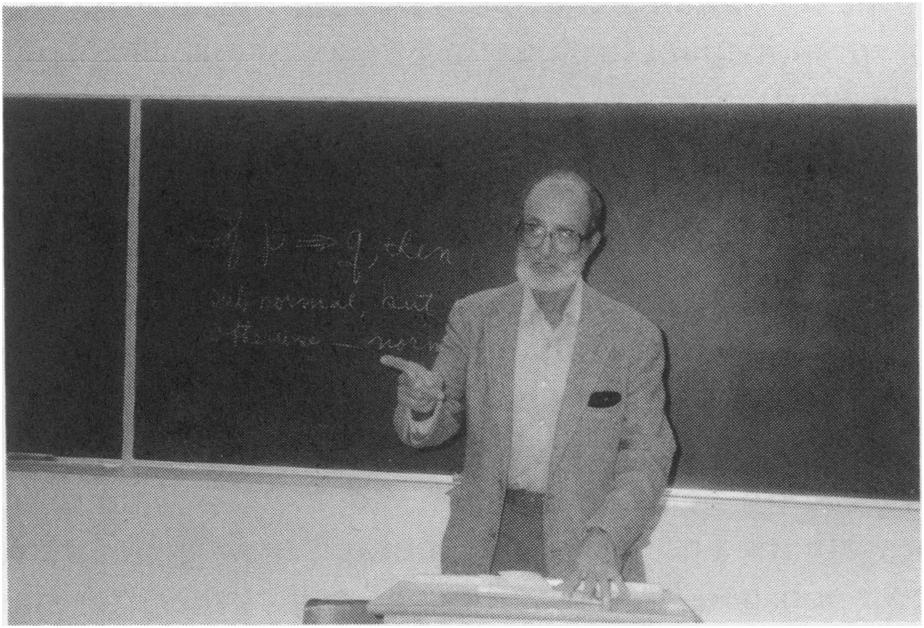
\includegraphics[width=.6\linewidth]{Halmos-Teaching.png}
\caption{\label{fig:halmos-teaching}Paul Halmos.}
\end{figure}

The method doesn’t begin by proving Theorem 1.  It begins with questions:
what is true, what do the examples we can look at suggest?  It doesn’t say
“look, here’s how it’s done”, it asks “how can it be done?”  It teaches
the right attitude toward the solution of all problems.  The problems that
we came here to solve can be solved—all problems can be solved—and the
teaching of problem solving is the way to set about solving them.  If we
could teach every teacher to teach every course as a problem course, then
one generation from now, in twenty five years, say, the need for talks
such as this one would no longer exist.  All we have to do is find out how
to do that, and we can adjourn.

Let me emphasize one thing I casually dropped along the way: I spoke of
the way to begin.  The way to begin all teaching is with a question.  I
try to remember that precept every time I begin to teach a course, and I
try even to remember it every time I stand up to give a lecture—and, you
may recall, I remembered it and acted on it today.

Another part of the idea of the method is to concentrate attention on the
definite, the concrete, the specific.  Once a student understands, really
and truly understands, why \(3 \times 5\) is the same as \(5 \times 3\),
then he quickly gets the automatic but nevertheless exciting and obvious
conviction that “it goes the same way” for all other numbers.  We all seem
to have an innate ability to generalize (shades of Chomsky again?).  The
teacher’s function is to call attention to a concrete special case that
hides (and, we hope, ultimately reveals) the germ of the conceptual
difficulty.

One time I used the so-called Moore method in an honors class in linear
algebra with about 15 students.  The first day of class I handed each
student a set of 19 pages stapled together and I told them that they now
held the course in their hands.  Those 19 pages contained the statements
of fifty theorems, and nothing else.  There were no definitions, there was
no motivation, there were no explanations—nothing but fifty theorems,
stated correctly but brutally, with no expository niceties.  That, I told
them, is the course.  If you can understand, state, prove, exemplify, and
apply those fifty theorems, you know the course, you know everything that
this course is intended to teach you.

I will not, I told them, lecture to you, and I will not prove the theorems
for you.  I’ll tell you, bit by bit as we go along, what the words mean,
and I might from time to time indicate what this subject has to do with
other parts of mathematics, but most of the classroom work will have to be
done by you.  I am challenging you to discover the proofs for yourselves, I
am putting you on your honor not to look them up in a book or get outside
help in any other way, and then I’ll ask you to present in class the
proofs you have discovered.  The rest of you, the ones who are not doing
the presenting, are supposed to stay on your toes mercilessly—make sure
that the speaker gives a correct and complete proof, and demand from the
speaker whatever else is appropriate for understanding (such as examples
and counterexamples.)

They stared at me, bewildered and upset—perhaps even hostile.  They had
never heard of such a thing.  They came here to learn something and now
they didn’t believe they would.  They suspected that I was trying to get
away with something, that I was trying to get out of the work I was paid
to do.  I told them about R. L. Moore, and they liked that, that was
interesting.  Then I gave them the basic definitions they needed to
understand the statements of the first two or three theorems, and said
“class dismissed”.

It worked.  At the second meeting of class I said, “O.K., Mr. Jones,
let’s see you prove Theorem 1”, and I had to push and drag them along
before they got off the ground.  After a couple of weeks they were
flying.  They liked it, they learned from it, and they entered into
the spirit of research—competition, discouragement, glory, and all.

If you are a teacher and a possible convert to the Moore method, don’t
make the mistake that my students made: don’t think that you, the teacher,
will do less work that way.  It takes me a couple of months of hard work
to prepare for a Moore course, to prepare the fifty theorems, or whatever
takes their place.  I have to chop the material into bite-sized pieces, I
have to arrange it so that it becomes accessible, and I must visualize the
course as a whole—what I can hope that they will have learned when it’s
over.  As the course goes along, I must keep preparing for each meeting:
to stay on top of what goes on in class, I myself must be able to prove
everything.  In class I must stay on my toes every second.  I must not
only be the moderator of what can easily turn into an unruly debate, but I
must understand what is being presented, and when something fishy goes on
I must interrupt with a firm but gentle “Would you explain that please?—I
don’t understand.”

Let me conclude by calling attention to a curious aspect of what I am
recommending, an aspect visible in my urging attention to the concrete
special case in order to understand the sweeping broad generalization.
In effect I am saying that we do not, we cannot understand a vacuum—what
we understand is always, in a sense, a fact—and, therefore, just as what
cannot be taught without how, and how cannot be taught without why, the
question has come full circle around to its start, and it turns out that
why cannot be taught without what.

Facts, methods, and insights—all are essential to all of us, all enter all
our subjects, and our principal job as teachers is to sort out the what,
the how, and the why, point the student in the right direction, and then,
especially when it comes to the why, stay out of his way so that he may
proceed full steam ahead.

Having expressed my strong views about why we should teach problem courses,
I call your attention to my major omission: I haven’t said a single word about how
to do that.  How, exactly, does one go about teaching a problem course in freshman
calculus, or, for that matter, in freshman rhetoric, or junior history, or graduate
astronomy?  I don’t pretend to know all the answers, but I have been working at
finding them for many years.  If you extended my lecture time by another hour or
so, or, to be more realistic, by another month or so, I could try to tell you about
some of the techniques that I have luckily blundered into.  My presentation today
was intended to touch briefly on the “why” of such teaching, not the “how”.  That
will have to wait for our next meeting—just tell me when and where it is, and I’ll
start packing my bag right away.
\end{document}

% Local Variables:
% TeX-engine: luatex
% End:
